\documentclass[11pt, a4paper]{article}
\usepackage{graphicx}
\usepackage[lofdepth,lotdepth]{subfig}
%opening
\title{A subfig csomag használata}
\author{Virágh János}
%
\begin{document}
\maketitle
\listoftables
\listoffigures
\section{Example with 3 "sub" tables}
\begin{table}[ht]
\centering
\subfloat[Subtable 1 list of tables text][Subtable 1 caption]{
\begin{tabular}{l|ccc}
& 1 & 2 & 3\\
\hline
1 & A & B & C\\
2 & D & E & F\\
\end{tabular}}
\qquad
\subfloat[Subtable 2 list of tables text][Subtable 2 caption]{
\begin{tabular}{l|ccc}
& 1 & 2 & 3\\
\hline
1 & A & B & C\\
2 & D & E & F\\
\end{tabular}}
\qquad
\subfloat[Subtable 3 list of tables text][Subtable 3 caption]{
\begin{tabular}{l|ccc}
& 1 & 2 & 3\\
\hline
1 & A & B & C\\
2 & D & E & F\\
\end{tabular}}
\caption{This is a table containing several subtables.}
\end{table}
\clearpage
\section{Example with 4 "sub" figures}
\begin{figure}[h]
\centering
\subfloat[Subfigure 1 list of figures text][Subfigure 1 caption]{

\includegraphics[width=0.25\textwidth]{Képek/Lion.pdf}
\label{fig:subfig1}}
\qquad
\subfloat[Subfigure 2 list of figures text][Subfigure 2 caption]{
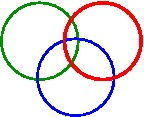
\includegraphics[width=0.35\textwidth]{Képek/korok.jpg}
\label{fig:subfig2}}
\subfloat[Subfigure 3 list of figures text][Subfigure 3 caption]{
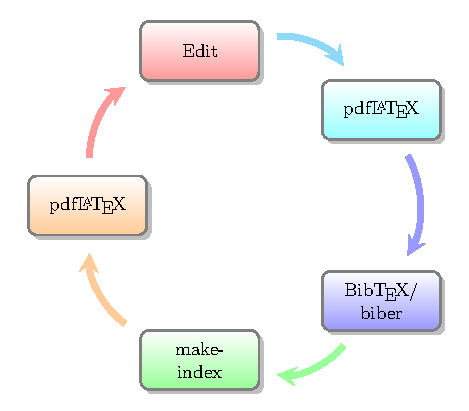
\includegraphics[width=0.35\textwidth]{Képek/smart-circle.pdf}
\label{fig:subfig3}}
\qquad
\subfloat[Subfigure 4 list of figures text][Subfigure 4 caption]{

\includegraphics[width=0.35\textwidth]{Képek/tiger.jpg}
\label{fig:subfig4}}
\caption{This is a figure containing several subfigures.}
\label{fig:globfig}
\end{figure}
In the text, you can refer to subfigures of figure \ref{fig:globfig} as \ref{fig:subfig1}, \ref{fig:subfig2}, \ref{fig:subfig3} and \ref{fig:subfig4} and to the sub-index as \subref{fig:subfig1}, \subref{fig:subfig2}, \subref{fig:subfig3} and \subref{fig:subfig4}.
\end{document}
